\chapter{Using the Hadoop Streaming Interface with Python}

\setcounter{problem}{1}

\begin{fullwidth}
{\em in progress}

\section{Goal}

Your goal in this lab is to learn how to launch a simple map-reduce job at Amazon using their elastic map reduce mechanism. Our application is the trite ``word counting,'' which we will use to find the most common words in a set of Google ads scarfed from the net in {\tt ads1000.txt} at github/parrt/msan501. You'll use Python as in the other labs.

\section{Discussion}

\section{Hadoop introduction}

Hadoop is written in Java and so to use another language, such as Python, we have to use the so-called {\em streaming interface}. That just means that we will write programs that read from standard input and write to standard output. Hadoop is a distributed computing framework that supports a \href{http://wiki.apache.org/hadoop/HadoopMapReduce}{\textcolor{blue}{map-reduce computing paradigm}}. The {\em map} operation executes on multiple machines and gets partial results, which are then combined with the {\em reduce} operation. 

The hadoop file system (HDFS) is a distributed file system that can handle massive amounts of data by distributing it across multiple machines and hard drives. Hadoop tries to keep map operations on the machines that store the associated data the mappers should run on. That is what typically is done, but we will be using Amazons S3 storage instead since it is the easiest thing to do.

Hadoop splits the input into chunks and gives each  chunk to a mapper, which generates partial results. Hadoop splits the input into lines before feeding it to standard input of the mappers. The mappers generate partial results as a set of key-value pairs of the form:

{\em key} \verb+\t+ {\em value} \verb+\n+

Hadoop sorts these according to key and distributes regions of the key space across one or more reducers. The reducer  reads these key-value pairs line by line and is responsible for generating the final result.  That output can be whatever we want, but in our case we will use the same output format. Because the partial results are created on a variety of machines where the map tasks ran, hadoop has to collect this data across the network before giving it to the reducers. Hadoop does a merge sort on these partial results.

We don't have to have any reducers at all, if we just want to run mappers across all the data.

We will be using Amazon Elastic MapReduce (EMR) that will take care of all the details of launching a cluster, running our job, and creating the output files.  A hadoop {\em job} is a chunk of work, which can have one or more tasks. If one of these tasks fails, hadoop tries to rerun them.  One of its big benefits is that it is fault-tolerant. In a cluster of 1000 computers, it's very possible machine will go down or the system operator will kick a power cord out by mistake. AWS introduces the notion of a {\em step}, which is one of more jobs. We will be using one step that consists of a mapper and reducer written in Python.

Hadoop streaming likes to generate an output file per reducer, which can be handy if we are interested in partitioning, say, sales results per country. In that case, we would have one reducer per country.  When I asked for three reducers, I got the following files in my output folder:

\scalebox{.65}{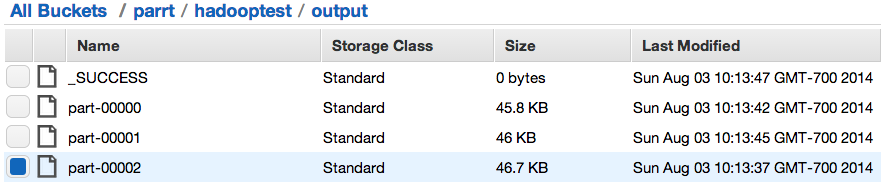
\includegraphics{figures/3reducers-output.png}}

To get a single output file, we need to specify a single reducer. Is a general warning, remember that this file should be small enough to fit easily on a single machine. {\em todo: try mapred.tasktracker.reduce.tasks.maximum=1 or mapred.reduce.tasks=1. With -D?}

\section{Testing map-reduce on single machine}

Before wasting money at Amazon to run your job, make sure that it works properly by simulating it from the command line on your laptop. To simulate hadoop collecting data and sending it as standard input to your mapper, we will use {\tt cat}:

\begin{alltt}\small
$ cat /tmp/ads1000.txt
"title"	"blurb"	"url"	"target"	"retrievetime"
"Exclusive Music For DJs"	"DJ One Stop For Edits, Mash-Ups, Remixes. Browse, Listen, Purchase!"	"www.StrictlyHits.com"	"http://www.strictlyhits.com"	"2009-08-28 02:48:01"
...
\end{alltt}

 We need to pipe this into the mapper

\begin{alltt}\small
$ cat /tmp/ads1000.txt | python wcmap.py
"title"	1
"blurb"	1
"url"	1
"target"	1
"retrievetime"	1
"Exclusive	1
Music	1
For	1
DJs"	1
"DJ	1
...
\end{alltt}

Hadoop always sorts the partial results coming out of each mapper before passing it to the reducer(s).

\begin{alltt}\small
$ cat /tmp/ads1000.txt | python wcmap.py | sort
!	1
!	1
!	1
!	1
!	1
!"	1
!"	1
!"	1
!"	1
...
\end{alltt}

Obviously the data is not very interesting because we have not stripped out punctuation, which you can do as an exercise.  The point is that the data is sorted by key. Then, we can run the reduce job:

\begin{alltt}\small
$ python wcmap.py < /tmp/ads1000.txt |sort| python wcreduce.py
...
\end{alltt}

The issue is that our Python program does not sort by keys when emitting key-value pairs, but we can use the command line to handle that. Here is our final command line that streams data using pipes between processes:

\begin{alltt}\small
$ python wcmap.py < /tmp/ads1000.txt |sort| python wcreduce.py | sort
!       5
!"      6
"#3     3
"$189   3
"$200   1
...
\end{alltt}

We can write that to file using:

\begin{alltt}\small
$ python wcmap.py < /tmp/ads1000.txt |sort| python wcreduce.py | sort
\end{alltt}

On a multicore machine, this process is virtually identical to what hadoop is doing for us, except of course on a smaller scale.

\section{S3 storage}

AWS's elastic map reduce mechanism likes to process data out of its S3 storage. You will need to create a bucket in S3 that is unique across AWS so maybe use your user ID. My bucket is parrt. And I can access that with web address: \href{https://parrt.s3.amazonaws.com}{\textcolor{blue}{parrt.s3.amazonaws.com}}. As long as I've made the folders underneath public, then I can add elements to the URL to get access to those files. For example, here is the data that I have updated for our lab in the msan501 bucket:

\href{http://msan501.s3.amazonaws.com/data/ads1000.txt}{\textcolor{blue}{http://msan501.s3.amazonaws.com/data/ads1000.txt}}

\section{Running the job}

The process of running a map reduce job is simple:

\step Load your data into an S3 bucket folder by downloading from msan501/data and uploading it into your own bucket.

\scalebox{.35}{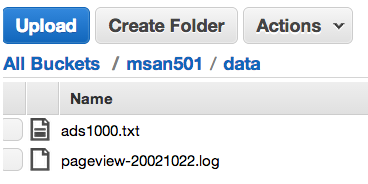
\includegraphics{figures/msan501-data.png}}

\step Load your code into S3, presumably in a different folder.

\scalebox{.35}{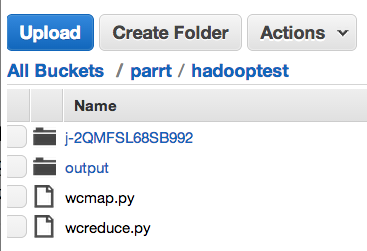
\includegraphics{figures/hadooptest.png}}

\step Create a job using EMR interface. Click on the ``Create cluster'' button. Choose all the defaults on the resulting page, except:

\begin{itemize}
\item Turn OFF ``Termination protection'' near the top.
\item Set a log dir like {\tt s3://parrt/hadooptest/logs} or something appropriate ({\em a directory that does not exist!}).
\item You can delete Hive and Pig ``Applications to be installed.''
\item Under Steps near the bottom, select ``Streaming program'' from the ``Add step'' drop-down. If you want to keep the cluster alive so that you can rerun jobs more quickly, set auto terminate to no. Otherwise set it to yes so that the cluster disappears after your job and you will not be charged further for it. We will the using three machines, one master and two core.
\end{itemize}

\step Enter the fields of the step dialogue as shown, substituting your user ID or your bucket/folder names as appropriate:

\noindent\scalebox{1.0}{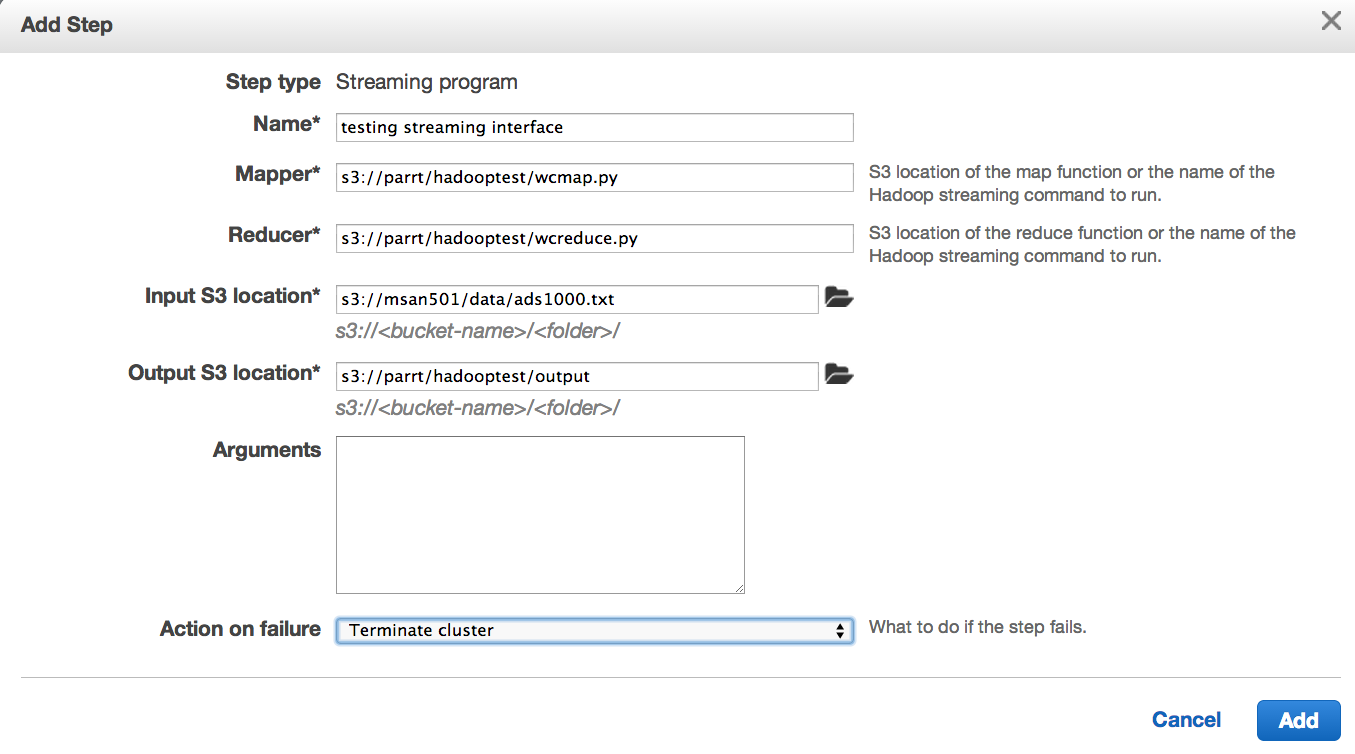
\includegraphics{figures/jobsetup.png}}

{\bf Warning!} If you launch a cluster and tell it to write to an existing directory, it will fail with a permissions issue and the cluster will terminate.  Consequently, use output directories with different names for each run.

For convenience, here is the text so that you can cut-and-paste:

\begin{alltt}\small
s3://parrt/hadooptest/wcmap.py
s3://parrt/hadooptest/wcreduce.py
s3://msan501/data/ads1000.txt
s3://parrt/hadooptest/output4
\end{alltt}

\step Wait about 15 minutes while Amazon creates the cluster and then you can wait a fraction of a second for to run the job.
\step Download or examine your data with the S3 interface.

If we have a cluster on which we have installed hadoop, we can run from the command line. The above is basically the same as:

\begin{alltt}\small
$ hadoop jar /home/hadoop/contrib/streaming/hadoop-streaming.jar \textbackslash
  -files s3://parrt/hadooptest/wcmap.py,s3://parrt/hadooptest/wcreduce.py \textbackslash
  -mapper wcmap.py -reducer wcreduce.py \textbackslash
  -input s3://msan501/data/ads1000.txt \textbackslash
  -output s3://parrt/hadooptest/output
\end{alltt}


Once our cluster is up, you can run another job ``quickly'' by adding another step. Go into EMR and select your cluster and then click "add step". That is a tiny link hidden down in the Steps area.

\section{Resources}

\begin{itemize}
\item You will find {\tt wcmap.py} and {\tt wcreduce.py} at github. There is also the necessary data file, {\tt ads1000.txt}.
\item \href{http://cs.smith.edu/dftwiki/index.php/Hadoop_Tutorial_3.2_--_Using_Your_Own_Streaming_WordCount_program}{\textcolor{blue}{A helpful tutorial}}, from which we get our sample programs.
\end{itemize}

\section{Deliverables}

None. Please follow along in class.

If you are feeling particularly frisky, you can improve the mapper so that it strips punctuation so that we get a much better set of keys. You can also strip characters not in the printable ASCII code.

\end{fullwidth}
